% Created 2022-01-22 Sat 19:58
% Intended LaTeX compiler: xelatex
\documentclass[10pt,twoside,landscape]{article}
\usepackage{graphicx}
\usepackage{longtable}
\usepackage{wrapfig}
\usepackage{rotating}
\usepackage[normalem]{ulem}
\usepackage{amsmath}
\usepackage{amssymb}
\usepackage{capt-of}
\usepackage{hyperref}
\usepackage[newfloat]{minted}
\usepackage{color}
\usepackage{listings}
\usepackage[top=2cm,bottom=2cm,right=2cm,left=2cm,landscape]{geometry}
\usepackage{multicol}
\usepackage{enumitem}
\setlist{noitemsep}
\setlength{\parindent}{0pt}
\setlength{\columnseprule}{0.2pt}
\definecolor{mygreen}{rgb}{0,0.6,0}
\definecolor{mygray}{rgb}{0.5,0.5,0.5}
\definecolor{mymauve}{rgb}{0.58,0,0.82}
\lstset{ backgroundcolor=\color{white}, basicstyle=\footnotesize, breaklines=true, captionpos=b, commentstyle=\color{mygreen}, escapeinside={\%*}{*)},keywordstyle=\color{blue}, stringstyle=\color{mymauve},}
\author{Olivier Lischer}
\date{\today}
\title{MGE WPF Summary}
\hypersetup{
 pdfauthor={Olivier Lischer},
 pdftitle={MGE WPF Summary},
 pdfkeywords={},
 pdfsubject={},
 pdfcreator={Emacs 27.2 (Org mode 9.5.2)}, 
 pdflang={English}}
\begin{document}

\begin{multicols}{4}

\textbf{Code Behind}

Every \href{../../../roam/20211123162923-wpf.org}{WPF} Window has a \href{../../../roam/20211123162058-xaml.org}{XAML} file for the graphical part and a \href{../../../roam/20211003114158-c.org}{C\#} (or any other \href{../../../roam/20211003114703-net.org}{.NET} language) file.
The code in the C\# file is called the Code Behind.
This file is used to implement the event handler.

\textbf{XAML}

\href{../../../roam/20211123162058-xaml.org}{XAML} short for Extensible Application Markup Language is \href{../../../roam/20211123161400-markup_language.org}{Markup Language} from \href{../../../roam/20211123161417-microsoft.org}{Microsoft} for creating graphical UIs.
XAML is based on \href{../../../roam/20211112100344-xml.org}{XML}.

\textbf{Code to EXE}

\begin{center}
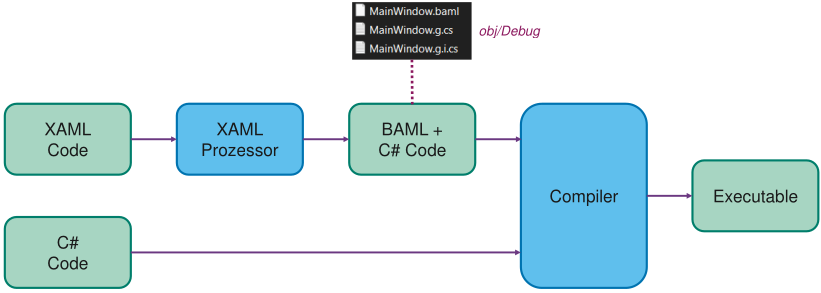
\includegraphics[width=.9\linewidth]{img/xaml_to_application.png}
\end{center}

\textbf{Logical View}

The Logical Tree is the representation of your \href{../../../roam/20211123162058-xaml.org}{XAML}.
Only the controls \textbf{you} define are shown in the Logical Tree.
In the figure only the green blocks are part of the Logical Tree.

\begin{center}
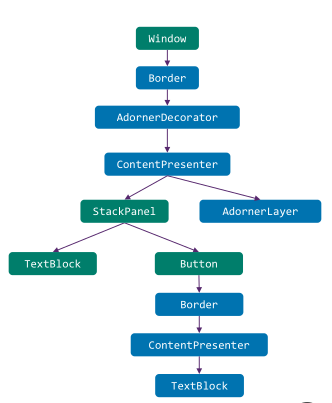
\includegraphics[width=.9\linewidth]{img/visual_logical_tree.png}
\end{center}

\textbf{Visual Tree}
The Visual Tree is the representation of your \href{../../../roam/20211123162058-xaml.org}{XAML} including the elements you don't specify.
The blue elements in the figure are added to the Tree.
This Blue elements are part of the default control of a type.
The Visual Tree in the figure is the whole tree.

\textbf{Namespaces - XAML}

In \href{../../../roam/20211123162058-xaml.org}{XAML} you can define / import namespaces using the \texttt{xmln} keyword.
Without a colon it is the default namespace.
With colon, you have to specify the prefix to use the elements form the namespace. 

\textbf{Standard Namespaces - XAML}

Some namespaces have some prefixes by conventions:
\begin{itemize}
\item default namespace points to the WPF Control Library
\item \texttt{x} points to \href{../../../roam/20211123162058-xaml.org}{XAML} specific elements
\item \texttt{d} point to elements which are only required for the visual designer
\item \texttt{mc} for elements of \emph{Markup Compatibility}
\item \texttt{local} for elements from you own assembly
\end{itemize}

!!Source 1!!

\textbf{Event Handler - XAML}

Every control has events.
In the \href{../../../roam/20211123162058-xaml.org}{XAML} you can just assign to the Name of the Event a string with name of the function / handler.
This function is in the code behind class implemented.

!!Source 2!!


\textbf{XAML Syntax's}

In XAML we have two different kind of syntax's:
\begin{itemize}
\item the Attribute Syntax
\item the Property Element Syntax
\end{itemize}

!!Source 3!!

\textbf{Content Propery - XAML}

Each \href{../../../roam/20211123162058-xaml.org}{XAML} element can specify exactly one property for its content.
This property can be set over \href{../../../roam/20211207160947-the_attribute_syntax_in_xaml.org}{The Attribute Syntax in XAML} or you write the value between the start and end tag.


\textbf{Attached Properties - XAML}

Attached Properties are used to set the property on an element, but the property belongs to another element (The property is attached).
This is mostly used in combination with Layouts.
This is similar the Properties in Android witch are prefixed with \texttt{layout\_}.

!!Source 4!!


\textbf{Type Converters}

Type Converters are used to convert a string into a complex type.
This is very often used to simplify the XAML.
To implement a custom type converter you have to inherit from \texttt{TypeConverter}

!!Source 5!!

\textbf{Markup Extensions - XAML}

Markup Extensions are used in the \href{../../../roam/20211123162058-xaml.org}{XAML} markup to use additional logic.
They are very common for styling and data binding.
To implement a custom Markup Extension you have to inherit from \texttt{MarkupExtension}.

!!Source 6!!

\textbf{Class Hierarchy}

\begin{center}
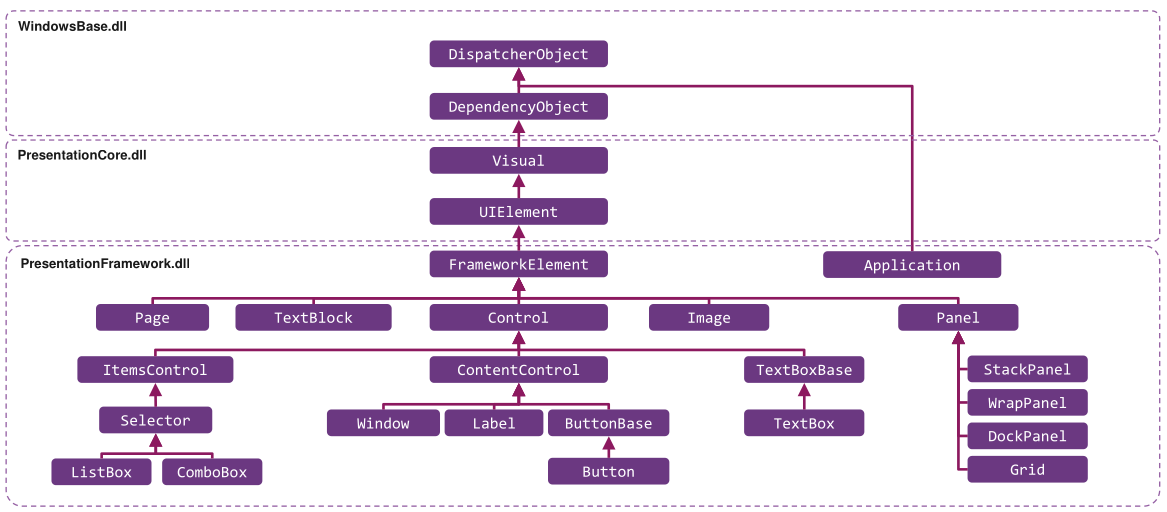
\includegraphics[width=.9\linewidth]{img/class_hierarchy.png}
\end{center}

TODO?!

\textbf{Dimensions}

\begin{itemize}
\item no unit = device independent pixels (DIP), 1in
\item px
\item in
\item cm
\item pt
\item Auto
\end{itemize}

Use only \texttt{Auto} and \texttt{DIP}.
\begin{itemize}
\item \texttt{n}: same value for all sides
\item \texttt{x,y}: x for horicontal , y for vertical
\item \texttt{l,t,r,b}: left, top, right, bottom
\end{itemize}

\textbf{Panels / Layout}

Panels / Layouts are Container for other child elements.
They are very similar to the Layouts in Android.
The panels could be nested, but you should not do this because of performance impacts.

\textbf{StackPanel}

It's a layout in the WPF.

\begin{center}
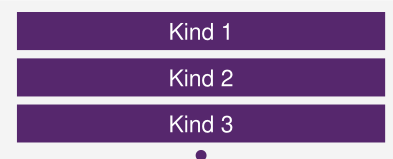
\includegraphics[width=.9\linewidth]{img/stack_panel_vertical.png}
\end{center}

!!Source 7!!

\textbf{WrapPanel}

It's a layout in the WPF.
If no space  is left, the next element is wrapped on the next line.

\begin{center}
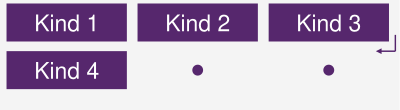
\includegraphics[width=.9\linewidth]{img/wrap_panel_horizontal.png}
\end{center}

!!Source 8!!

\textbf{DockPanel}

It's a layout in the WPF.
The last element fills the remaining space.
You can prevent this behavior using \texttt{LastChildFill ="False"}.

\begin{center}
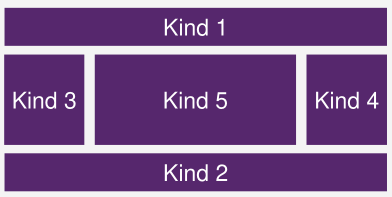
\includegraphics[width=.9\linewidth]{img/dockpanel_version_one.png}
\end{center}

!!Source 9!!

\textbf{Grid}

It's a layout in the WPF.
Using \texttt{RowSpan} and \texttt{ColSpan} multiple Rows / Columns can be merged into one.

\begin{center}
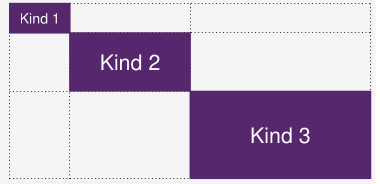
\includegraphics[width=.9\linewidth]{img/grid_layout.png}
\end{center}

!!Source 10!!

\textbf{Resources in XAML}

Every object which could be described in XAML (Brush, Color, String) could be a resource.
A resource is similar to a variable in \href{../../../roam/20211003114158-c.org}{C\#} code.
Every resource has a unique ID (\texttt{x:Key}).

\textbf{Resource Dictionary}

A Resource Dictionary is a container (key-value) to store resources.
The attribute \texttt{x:Key} is the key.
A local Resource Dictionary is available on all Elements inheriting from \texttt{FrameworkElement}.
The \texttt{Application} class is used for global resources.

The Resource Dictionary is access over the Property Element Syntax.

!!Source 11!!

\textbf{Resource Search Order}

Search Order for Resources:
\begin{enumerate}
\item In the Logical-Tree from bottom to top
\item In \textbf{Application.Resources}
\item In \textbf{System.Ressourcen}
\end{enumerate}

The search is abort at the first hit.
If the Key is not found a Runtime-Exception is thrown.

\textbf{Static Resources}

Static Resources are only evaluated once during the compile time.
During the runtime it is not possible to change its value.

!!Source 11!!

\textbf{Dynamic Resources}

Dynamic Resources can be evaluated multiple times.
The evaluation is during the runtime and is updated when the value is changed.

!!Source 11!!

\textbf{Resource Dictionary in other file}

Sometimes you want to extract your Resource Dictionary into a separate \href{../../../roam/20211123162058-xaml.org}{XAML} file.
This file contains the \texttt{<ResourceDictionary>} tag as \href{../../../roam/20211112100344-xml.org}{XML} root.
In the other file you can include separate XAML file using \texttt{MergedDictionaries}:

!!Source 14!!

\textbf{Access static C\# from XAML}

Sometimes you have to access static values in the \href{../../../roam/20211003114158-c.org}{C\#} code.
For example constants from \href{../../../roam/20211003114703-net.org}{.NET} or form your own code.
You can access the value over th markup extension \texttt{x:Static}.

!!Source 15!!

\textbf{Styles in WPF}

Styles are a \href{../../../roam/20211123162058-xaml.org}{XAML} object which group multiple setters together.
The style can be used inside a Resource Dictionary.

Without styles, you have to set every property, for example the background, on each element.
This leads to code duplication.

!!Source 17 / 18!!

\textbf{Explicit Styles}

Explicit Styles required the property \texttt{x:Key}.
!!Source 17!!

\textbf{Implicit Styles}

Implicit Styles must not have the property \texttt{x:Key} explicit set.
But requires the property \texttt{TargetType}.
The property \texttt{x:Key} gets automatically the value \texttt{x:Key ="\{x:Type <Type>\}}
!!Source 18!!

\textbf{Extend your styles}

You can specify a base style, for example for your buttons.
Then you have two possibilities to extend your style:
\begin{enumerate}
\item Assign the style to the target type and set the specific Properties manually on the element
\item Create a new style which is based on the base style.
\end{enumerate}

!!Source 19!!

\textbf{Triggers in WPF}

Triggers allow you to modify your styling of an element based on its state.

!!Source 20!!

\textbf{Themes in WPF}

\href{../../../roam/20211123162923-wpf.org}{WPF} does not know the concept of skins / themes.
But using Resource Dictionaries this concept could be created.
The desired theme / resource dictionary is loaded at runtime using \texttt{DynamicResource}.


\textbf{Control Templates}

Control Templates are used to describe how a control should be display \(\rightarrow\) which element should be inserted in the \href{../../../roam/20211123163209-what_is_the_visual_tree_in_wpf.org}{What is the Visual Tree in WPF?}.
You can access the current template using the attribute \texttt{Control.Template}.

\textbf{Define Custom Control Template}

You can define the custom Control Template:
\begin{itemize}
\item as a Resource
\item inside a style
\end{itemize}


The attribute \texttt{ContentPrester} is used to define which attribute is used for the content.
The markup extension \texttt{TemplateBinding} is used to bind attributes.
This markup extension can only be used inside the Control Template.

\textbf{GUI Guidelines}

\href{../../../roam/20211123162923-wpf.org}{WPF} does not have any guidelines like Android.
However, you could / should use the same guidelines / libraries which are used in other places.
\begin{itemize}
\item \href{https://github.com/MaterialDesignInXAML/MaterialDesignInXamlToolkit}{Material Design in XAML}
\item \href{https://mahapps.com/docs/guides/quick-start}{MahApps.Metro}
\end{itemize}

\textbf{Data Binding}

Data Binding in \href{../../../roam/20211123162923-wpf.org}{WPF} works similar to the Data Binding in Android.
In WPF you use the markup extension \texttt{Binding} to bind property from the code behind.
To make the data from the code behind available for the \href{../../../roam/20211123162058-xaml.org}{XAML} you have to set the \texttt{this.DataContext}.

\textbf{Binding Types}

In \href{../../../roam/20211123162923-wpf.org}{WPF} exist three different biding types:
\begin{itemize}
\item \texttt{Binding} for 1:1 linking
\item \texttt{MultiBinding} for 1:n linking
\item \texttt{PriorityBinding} for 1:n / 1:1 linking
At the start the first source which response is used (turns a 1:n to 1:1 linking)
\end{itemize}

\textbf{Binding Properties}

A Binding object in WPF has the following properties:
\begin{itemize}
\item \texttt{Path}: Name of the source property
\item \texttt{Mode}: Direction of the data flow
\item \texttt{Converter}: Conversion between source and destination.
Is only used in Binding.
It is not the same as type converters.
\end{itemize}

\textbf{Binding Modes}

\begin{itemize}
\item \texttt{OneTime}: One-time update (very efficient, because no monitoring of the elements)
\item \texttt{OneWay}: Destination is updated when source is changed
\item \texttt{OneWaytoSource}: Source is updated when destination is changed (input fields)
\item \texttt{TwoWay}: Changes are propagated in both ways
\item \texttt{Default}: Value depends on destination property
\end{itemize}

!!Source 22!!

\textbf{Value Converter}

The Value Converter is a support object used in data binding in WPF.
The Value Converter converts the between source and destination so that it can be displayed on a from.
It also converts the value from an input field back to the class representation.

\textbf{Value Converter Implementation}

To implement a Value Converter you must implement the \texttt{IValueConverter} interface.
The \texttt{IValueConveter} interface provides the following methods:
\begin{itemize}
\item \texttt{Convert()}: Convert from source to destination
\item \texttt{ConvertBack()}: Convert from destination into source
\end{itemize}


For a multi binding converter you must implement the \texttt{IMultiValueConverter} interface.
The Value Converter can be created:
\begin{itemize}
\item as a resource
\item in code
\end{itemize}


!!Source 23!!

\textbf{Multi Binding}

Multi Binding is a special case of the Data Binding.
In contrast to normal Data Binding multi binding can bind multiple source properties.

!!Source 24!!

\textbf{DataContext}

The \texttt{DataContext} is used to define the default source for data binding.
If the \texttt{DataContext} is not set the logical tree is traversed to the top.

Even it is possible to set the \texttt{DataContext} for single elements this is not very common.
Normally you have one \texttt{DataContext} for one Window.


\textbf{WPF Element as Source}

Using the markup extension \texttt{RelativeSource} you refer to elements in the visual tree.
Try to avoid this markup extension because it is difficult to read and complex.
The markup extension \texttt{ElementName} can be used to refer to elements by their name.

!!Source 25!!

\textbf{Notify UI about data changes}

For Data Binding in WPF you can use any object as model.
However, the UI will not react on model changes.
To notify the UI you have to implement the \texttt{INotifyPropertyChanged} interface.
During the creation of the binding the destination register itself on the Event \texttt{PropertyChanged}
If the property is changed the Event is fired and the UI can be updated.

!!Source 26!!

\textbf{IL Weaving}

Using IL Weaving you modify the IL Code (\href{../../../roam/20211003114528-microsoft_intermediate_language.org}{MSIL}) at compile time.
This should only be used in exceptional cases because debugging is damn hard.

\textbf{Data binding using collections}

To bind a Collection to the UI you have to use a special collection type: \texttt{ObservableCollection<T>}.
This collection must be filled and then as the DataContext set.

The \texttt{ObservableCollection<T>} implements the \texttt{INotifyCollectionChanged} interface.
This notifies the UI only if the collection is changed (add / remove).
The model itself should implement the \texttt{INotifyPropertyChanged} interface.
Otherwise, the changes on the model are not reflected on the UI.

The model does not have to implement the \texttt{INotifyPropertyChanged} interface.
But normally it should.

To display the data inside the collection the \texttt{ItemTemplate} and \texttt{DataTemplate} must be overwritten (see example).

\textbf{Selectors for Collection in Data binding}
\begin{itemize}
\item \texttt{SelectedIndex}: Index in Collection
\item \texttt{SelectedItem}: Element as Object
\item \texttt{SelectedValue}: Selected Value
\item \texttt{SelectedValuePath}: Object path to the value which is returned in \texttt{SelectedValue}
\end{itemize}

!!Source 27!!

\textbf{MVVM}

The MVVM Pattern consists of three parts:
\begin{itemize}
\item \emph{Model}: contains the Domain / business logic
\item \emph{View}: contains the graphical UI and user input
\item \emph{View Model}: contains the logic form the UI and ensures the communication between Model and View
\begin{itemize}
\item This is often achieved over Data Binding
\end{itemize}
\end{itemize}


The benefits of the MVVM pattern are:
\begin{itemize}
\item View Model is easy to test because it does not contain any UI classes
\item the View has only visual tasks
\item Changes in the Model do not directly affect the View
\end{itemize}

\begin{center}
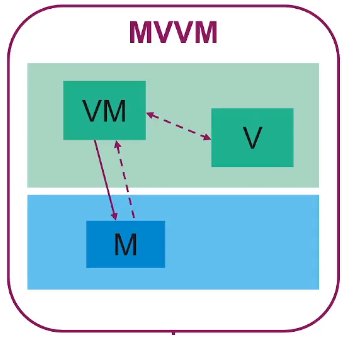
\includegraphics[width=.9\linewidth]{img/mvvm.png}
\end{center}

\textbf{ViewModel in WPF}
!!Source 28!!

\textbf{Bind Action to ViewModel}

Using Data Binding you can only bind properties.
Therefore methods must be packed in a object.
For this the \texttt{ICommand} interface is used.
!!Source 29!!

\textbf{RelayCommand}

The \texttt{RelayCommand} implements the \texttt{ICommand} interface and can be used to implement the actions directly on the ViewModel.
It is an alternative to the normal \texttt{ICommand} usage.
!!Source 30!!

\textbf{Rule of Thumb MVVM}

\begin{center}
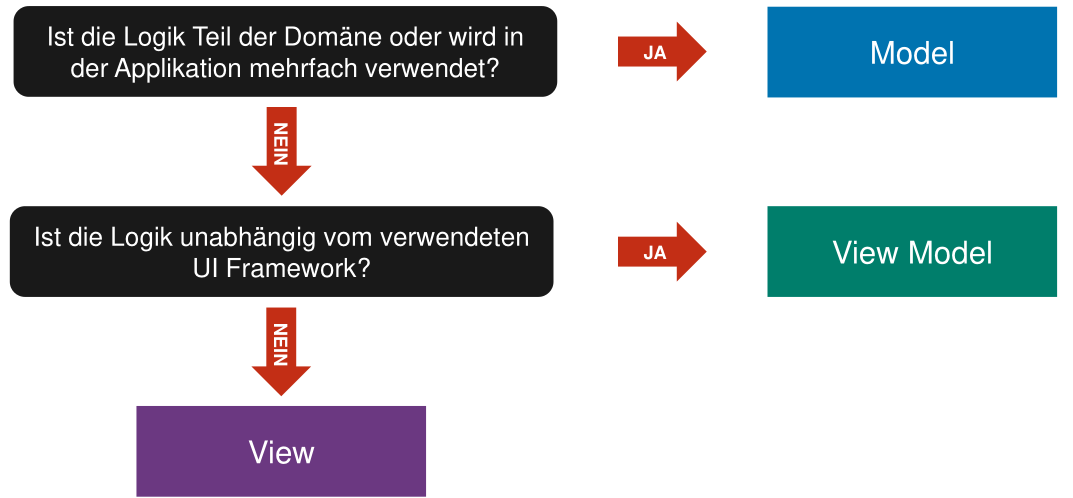
\includegraphics[width=.9\linewidth]{img/rule_of_thumb_logic_in_mvvm_.png}
\end{center}

\textbf{Separation in Software Engineering}

The Horizontal approach is the traditional one.
Changing the technology is easier.
This approach is used when each team works on one technology.

The Vertical approach is the modern approach.
It fits best for features teams.
Changing the technology can be difficult when everywhere should be used the same technology.

\begin{center}
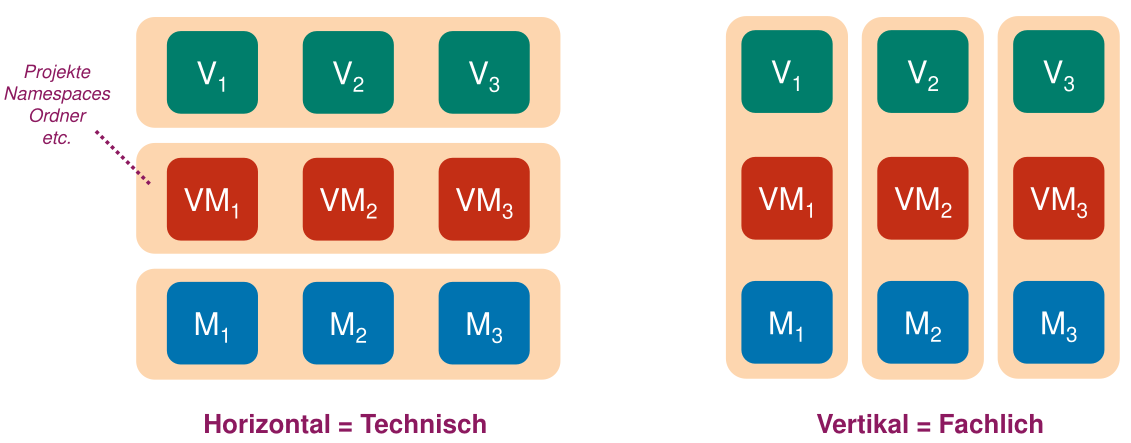
\includegraphics[width=.9\linewidth]{img/horizontal_vertical_cuts.png}
\end{center}

\textbf{Dependency Inversion Principle}

DIP = Dependency Inversion Principle

\begin{quote}
One should depend upon
abstractions, [not] concretions.

-- Robert C. Martin
\end{quote}

You want to implement against
\begin{itemize}
\item abstract classes
\item interfaces
\item delegates
\end{itemize}


You would never solder a lamp directly to the electrical wiring.

\textbf{Localization in WPF}

In \href{../../../roam/20211123162923-wpf.org}{WPF} you can create localization using
\begin{itemize}
\item Resources
\item over RESX files (recommended)
\end{itemize}


In general, it is a good idea to create a \emph{Translation Service} for the access in \href{../../../roam/20211003114158-c.org}{C\#} code.
With this approach the translation is technology independent.

\begin{center}
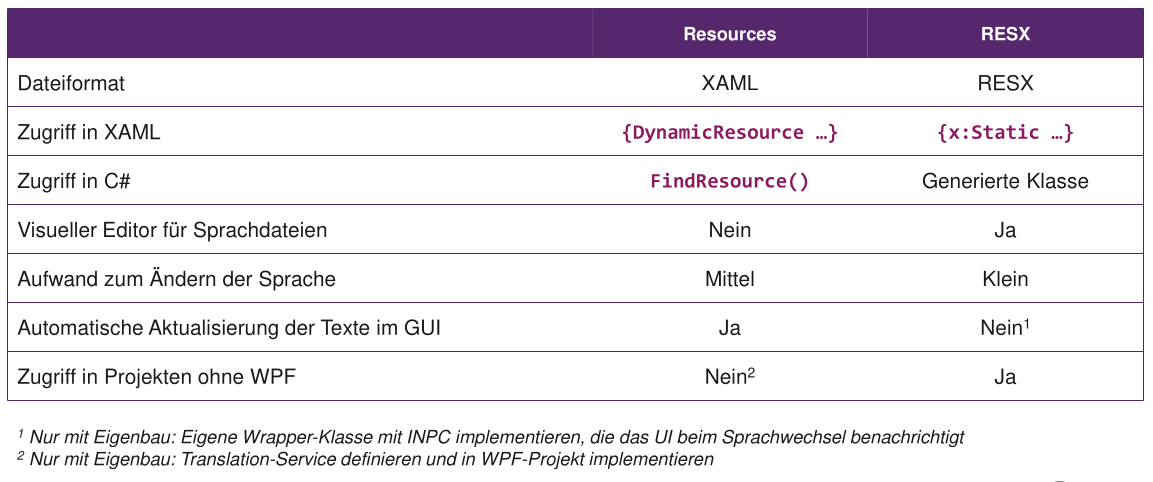
\includegraphics[width=.9\linewidth]{img/localization_wpf.png}
\end{center}

\textbf{Routed Events}

A UI Event in \href{../../../roam/20211123162923-wpf.org}{WPF} moves in two phases through the Visual Tree:
\begin{itemize}
\item \emph{Tunneling}: Top to bottom to focused element
\item \emph{Bubbeling}: Bottom to top from focused element
\end{itemize}


The traversing can be stopped at any element.
You only have to set \texttt{RoutedEventArgs.Handled} to \texttt{false}.


\begin{center}
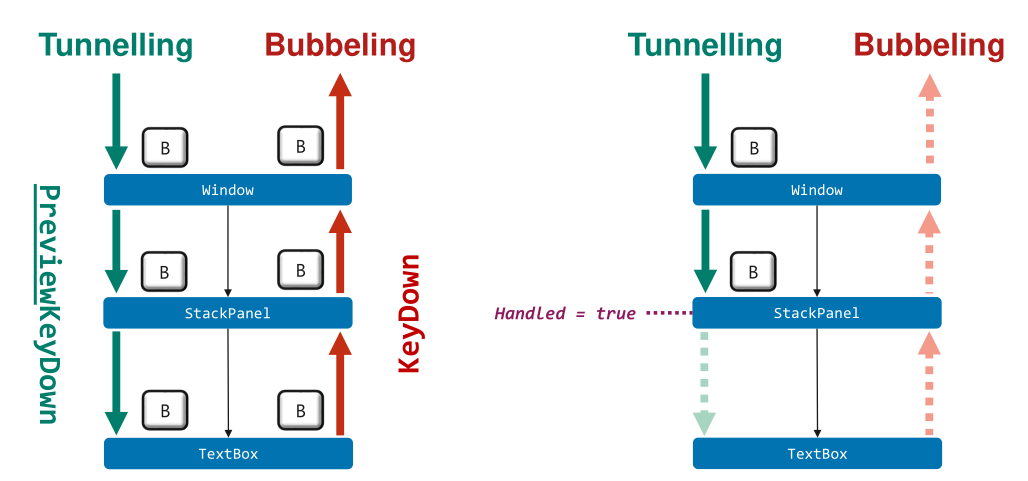
\includegraphics[width=.9\linewidth]{img/routed_events.png}
\end{center}


\textbf{Custom Controls / User Controls}

A Custom Control extends an already existing control.
The User Control is a composition from two existing controls.

In practice the custom control are more common because you have more control over it (styling).
The User Control can also be achieved with Custom Control.
You only have to overwrite the Control Template.


\begin{center}
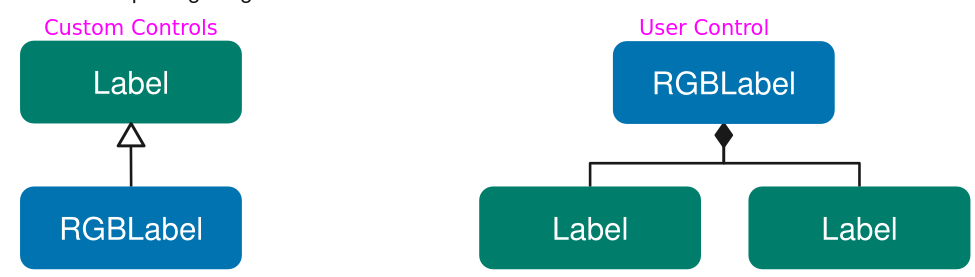
\includegraphics[width=.9\linewidth]{img/custom_user_control.png}
\end{center}

\textbf{Threading Model}

Every \href{../../../roam/20211123162923-wpf.org}{WPF} application has minimal two threads:
\begin{itemize}
\item UI Thread: Manages UI, receives events, execute actions
\item Rendering Thread: runs in background, draws controls
\end{itemize}


Thanks to this mechanism, controls are draw event when the UI Thread is blocked.
Only the UI Thread is allowed to change the UI.

!!Source 31!!

\textbf{UI update from background thread}

In \href{../../../roam/20211123162923-wpf.org}{WPF} only the UI Thread is allowed to update the UI.
Using a Dispatcher you can run an operation on the UI Thread from the background.
In a WPF Project you can access the dispatcher:
\begin{itemize}
\item Code Behind: \texttt{this.Dispatcher}
\item Other classes: \texttt{Application.Current.Dispather}
\end{itemize}


Data Binding does the dispatching automatically.
But the \texttt{ICommand.CanExecuteChanged} Event must be dispatched manually.
This could be done if you extend the RelayCommand.
!!Source 32!!

\textbf{Xamarin}

Xamarin is used to write apps in \href{../../../roam/20211003114158-c.org}{C\#} / \href{../../../roam/20211003114238-f.org}{F\#} for:
\begin{itemize}
\item \href{../../../roam/20210921143632-aosp.org}{Android Open Source Project}
\item \href{../../../roam/20220103094421-ios.org}{iOS}
\item \href{../../../roam/20220103094441-ipados.org}{iPadOS}
\item \href{../../../roam/20220103094458-watchos.org}{watchOS}
\item \href{../../../roam/20220103094511-tvos.org}{tvOS}
\item \href{../../../roam/20220103094529-macos.org}{macOS}
\end{itemize}


During the compilation \href{../../../roam/20210921091753-native_apps.org}{Native apps} are created.
When compiled for Android the \href{../../../roam/20211003114703-net.org}{.NET} Runtime is packed together.
So the runtime runs a runtime which runts the app.


\begin{center}
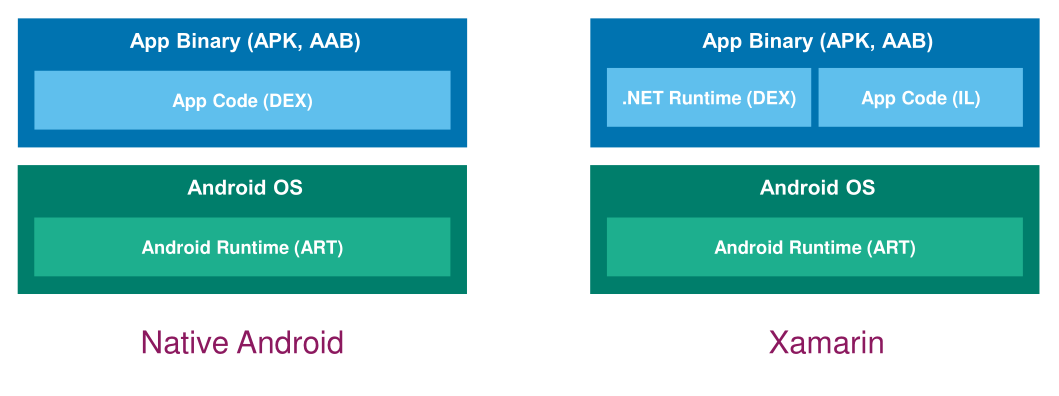
\includegraphics[width=.9\linewidth]{img/xamarin_native_android.png}
\end{center}

\textbf{Xamarin Structure}

You have \emph{Shared Code} and \emph{Platform Code}.
The Shared Code should be as big as possible while the platform code should be as small as possible.


\begin{center}
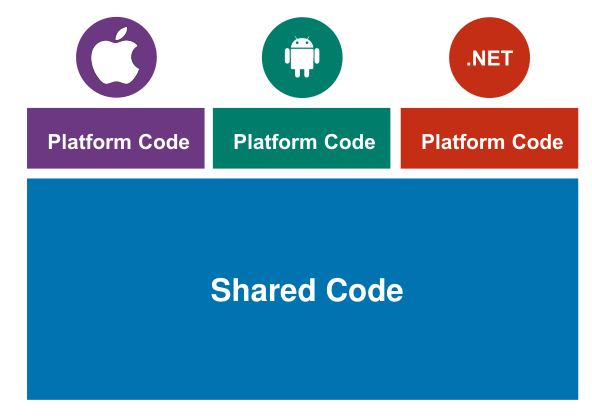
\includegraphics[width=.9\linewidth]{img/shared_platform_code.png}
\end{center}

\textbf{Xamarin Essentials}

Xamarin.Essentials is a collection of platform services like:
\begin{itemize}
\item Sensors (battery, \ldots{})
\item Interfaces (permissions, phone, \ldots{})
\item Utilities (Threading, conversion, \ldots{})
\end{itemize}


It is one interface for all platform.

\textbf{Xamarin Traditional}

In Xamarin Traditional you write the definition for the UI for each target platform using the native concepts.
The benefits are that it is faster, and you have total access to the underlying SDK.
The drawback is you have to write the same UI for each platform.

\textbf{Xamarin.Forms}

In Xamarin.Forms you write the UI as a part of the shared code using \href{../../../roam/20211123162058-xaml.org}{XAML}.
The benefit is you write the UI only once.
The drawback is you have some limitations in the design of the UI and slightly slower performance then Native.

However, in general you should use Xamarin.Forms instead of Xamarin Traditional.

\textbf{Xamarin Renderer}

\href{../../../roam/20220103094320-xamarin.org}{Xamarin} has many controls for example the button.
Render classes are used to map the Xamarin Button to the platform specific buttons.
Using Renderer you can adjust the styling.
You can also write custom renderers for existing controls and for custom \href{../../../roam/20211123162058-xaml.org}{XAML} Controls.


\begin{center}
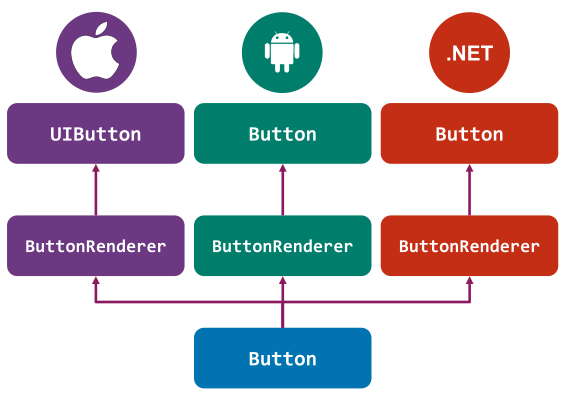
\includegraphics[width=.9\linewidth]{img/xamarin_renderer.png}
\end{center}

\end{multicols}
\begin{multicols}{2}
\section{Code}
\label{sec:org566124e}
\textbf{Source 1 - Default Namespaces}
\lstset{language=XML,label= ,caption= ,captionpos=b,numbers=none}
\begin{lstlisting}
<Window xmlns="http://schemas.microsoft.com/winfx/2006/xaml/presentation"
	xmlns:x="http://schemas.microsoft.com/winfx/2006/xaml"
	xmlns:d="http://schemas.microsoft.com/expression/blend/2008"
	xmlns:mc="http://schemas.openxmlformats.org/markup-compatibility/2006"
	xmlns:local="clr-namespace:Vorlesung_09"
	mc:Ignorable="d" <!-- Tells XAML that d should not be used during compilation -->
	/>
\end{lstlisting}

\textbf{Source 2 - Event Handlers}
\lstset{language=XML,label= ,caption= ,captionpos=b,numbers=none}
\begin{lstlisting}
<Button Click="MyButton_OnClick" Text="Click Me!" />
\end{lstlisting}

\lstset{language=csharp,label= ,caption= ,captionpos=b,numbers=none}
\begin{lstlisting}
void MyButton_OnClick(object sender, RoutedEventArgs evtArgs) {}
\end{lstlisting}

\textbf{Source 3 - XAML Syntax's}
\lstset{language=XML,label= ,caption= ,captionpos=b,numbers=none}
\begin{lstlisting}
<!-- Attribute Synatx -->
<Button Content="Mein Button"/>

<!-- Propery Element Synax -->
<Button>
  <Button.Background>
    <SolidColorBrush Color="Blue"/>
  </Button.Background>
  <Button.Content>
    Mein Button
  </Button.Content>
</Button>
\end{lstlisting}


\textbf{Source 4 - Attached Properties}
\lstset{language=XML,label= ,caption= ,captionpos=b,numbers=none}
\begin{lstlisting}
  <Grid>
    <Grid.RowDefinitions>
      <RowDefinition Height="30" />
    </Grid.RowDefinitions>
    <TextBlock Grid.Row="0" Name="G" Background="Green" />
</Grid>
\end{lstlisting}

\textbf{Source 5 - Type Converter}
\lstset{language=XML,label= ,caption= ,captionpos=b,numbers=none}
\begin{lstlisting}
<local:LocationControl Center="10, 20" />
\end{lstlisting}

\textbf{Source 6 - Markup Extensions}
\lstset{language=XML,label= ,caption= ,captionpos=b,numbers=none}
\begin{lstlisting}
<TextBlock Text="{local:LocationExtension Lat=10,Long=20}" />
\end{lstlisting}

\lstset{language=csharp,label= ,caption= ,captionpos=b,numbers=none}
\begin{lstlisting}
public class LocationExtension : MarkupExtension
{
    public string Lat { get; set; }
    public string Long { get; set; }
    public override object ProvideValue(IServiceProvider s)
    {
	return this.Lat + " / " + this.Long;
    }
}
\end{lstlisting}

\textbf{Source 7 - StackPanel}
\lstset{language=XML,label= ,caption= ,captionpos=b,numbers=none}
\begin{lstlisting}
<!-- Orientation could be Vertical or Horiztonal -->
<StackPanel Orientation="Vertical">
</StackPanel>
\end{lstlisting}

\textbf{Source 8 - WrapPanel}
\lstset{language=XML,label= ,caption= ,captionpos=b,numbers=none}
\begin{lstlisting}
<!-- Orientation could be Vertical or Horiztonal -->
<WrapPanel Orientation="Horizontal">
</WrapPanel>
\end{lstlisting}

\textbf{Source 9 - DockPanel}
\lstset{language=XML,label= ,caption= ,captionpos=b,numbers=none}
\begin{lstlisting}
<!-- Top | Bottom | Left | Right -->
<DockPanel>
  <TextBlock DockPanel.Dock="Top" />
  <TextBlock DockPanel.Dock="Left" />
</DockPanel>
\end{lstlisting}

\textbf{Source 10 - Grid}
\lstset{language=XML,label= ,caption= ,captionpos=b,numbers=none}
\begin{lstlisting}
<Grid>
  <Grid.RowDefinitions>
    <RowDefinition Height="1*" />
    <RowDefinition Height="2*" />
  </Grid.RowDefinitions>
  <Grid.ColumnDefinitions>
    <ColumnDefinition />
  </Grid.ColumnDefinitions>
  <TextBlock Grid.Row="0" Grid.Column="0" />
</Grid>
\end{lstlisting}

\textbf{Source 11 - Resource Dictionary}
\lstset{language=XML,label= ,caption= ,captionpos=b,numbers=none}
\begin{lstlisting}
<Window>
  <Window.Resources>
    <SolidColorBrush x:Key="OSTBrush" Color="#6E1C50" />
  </Window.Resources>
  <Label Content="Variante 1" Foreground="White">
    <Label.Background>
      <StaticResource ResourceKey="OSTBrush" />
    </Label.Background>
  </Label>
  <Label Content="Variante 2"
	 Foreground="White"
	 Background="{StaticResource ResourceKey=OSTBrush}" />
  <Label Content="Variante 3"
	 Foreground="White"
	 Background="{StaticResource OSTBrush}" />
  <Label Content="Variant 4"
	 Foreground="White"
	 Background="{StaticResource OSTBrush}" />
</Window>
\end{lstlisting}

\lstset{language=csharp,label= ,caption= ,captionpos=b,numbers=none}
\begin{lstlisting}
private void UpdateResource(object sender, RoutedEventArgs e)
{
    Resources["OSTBrush"] = new SolidColorBrush(Colors.Blue);
}
\end{lstlisting}

\textbf{Source 14 - Additional Resource Dictionary}
\lstset{language=XML,label= ,caption= ,captionpos=b,numbers=none}
\begin{lstlisting}
<!-- MyDictionary.xaml -->
<ResourceDictionary>
  <SolidColorBrush x:Key="OSTBrush2" Color="#6E1C50" />
</ResourceDictionary>

<!-- MyForm.xaml -->
<Window>
  <Window.Resources>
    <ResourceDictionary>
      <SolidColorBrush x:Key="OSTBrush" Color="#6E1C50" />
      <ResourceDictionary.MergedDictionaries> <!-- Include -->
	<ResourceDictionary Source="MyDictionary.xaml"/>
      </ResourceDictionary.MergedDictionaries>
    </ResourceDictionary>
  </Window.Resources>
  <Label Content="Externe Resource"
	 Foreground="White"
	 Background="{StaticResource OSTBrush2}" />
</Window>
\end{lstlisting}

\textbf{Source 15 - Static C\# Values}
\lstset{language=csharp,label= ,caption= ,captionpos=b,numbers=none}
\begin{lstlisting}
public static class MyRes
{
    public static readonly SolidColorBrush OSTBrush =
	new(Color.FromRgb(110, 28, 80));
}
\end{lstlisting}

\lstset{language=XML,label= ,caption= ,captionpos=b,numbers=none}
\begin{lstlisting}
<Label Content="x:Static"
       Background="{x:Static local:MyRes.OSTBrush}"
       Foreground="{x:Static SystemColors.ControlLightBrush}"
       FontFamily="{x:Static SystemFonts.CaptionFontFamily}"
       FontSize="{x:Static SystemFonts.CaptionFontSize}" />
\end{lstlisting}

\textbf{Source 17 - Explicit Styles}
\lstset{language=XML,label= ,caption= ,captionpos=b,numbers=none}
\begin{lstlisting}
<Window>
  <Window.Resources>
    <!-- TargetType is optional when used explicitly -->
    <Style x:Key="MyButtonStyle" TargetType="Button>
      <Setter Property="Button.Background" Value="Blue" />
      <Setter Property="Button.Foreground" Value="Black" />
      <Setter Property="Button.BorderBrush" Value="Black" />
      <Setter Property="Button.BorderThickness" Value="1" />
    </Style>
  </Window.Resources>
  <StackPanel>
    <Button Style="{StaticResource MyButtonStyle}"
	    Content="OK" />
    <Button Style="{StaticResource MyButtonStyle}"
	    Content="Cancel" />
  </StackPanel>
</Window>
\end{lstlisting}

\textbf{Source 18 - Implicit Style}
\lstset{language=XML,label= ,caption= ,captionpos=b,numbers=none}
\begin{lstlisting}
<Window>
  <Window.Resources>
    <!-- TargetType required -->
    <Style TargetType="Button>
      <Setter Property="Button.Background" Value="Blue" />
      <Setter Property="Button.Foreground" Value="Black" />
      <Setter Property="Button.BorderBrush" Value="Black" />
      <Setter Property="Button.BorderThickness" Value="1" />
    </Style>
  </Window.Resources>
  <StackPanel>
    <Button Content="OK" /> <!-- No style assigned -->
    <Button Content="Cancel" />
  </StackPanel>
</Window>
\end{lstlisting}


\textbf{Source 19 - Extended Style}
\lstset{language=XML,label= ,caption= ,captionpos=b,numbers=none}
\begin{lstlisting}
<!-- (1) combination approach -->
<Button Style="{StaticResource NormalButton}"
	Background="Red"
	Content="Cancel" />

<!-- (2) based on approach -->
<Window.Resources>
  <Style x:Key="NormalButton" TargetType="Button">
    ...
  </Style>
  <Style x:Key="DangerButton"
	 BasedOn="{StaticResource NormalButton}" <!-- here you inhert from NormalButton -->
	 TargetType="Button">
    <Setter Property="Background" Value="Red" />
  </Style>
</Window.Resources>
...
<Button Style="{StaticResource DangerButton}"
	Content="Cancel" />
\end{lstlisting}

\textbf{Source 20 - Triggers}
\lstset{language=XML,label= ,caption= ,captionpos=b,numbers=none}
\begin{lstlisting}
<Window.Resources>
  <Style x:Key="TriggerButton" TargetType="Button">
    <Style.Triggers>
      <Trigger Property="Content" Value="Edit">
	<Setter Property="Cursor" Value="Pen" />
      </Trigger>
    </Style.Triggers>
  </Style>
</Window.Resources>
<Button Style="{StaticResource TriggerButton}" Content="Edit" />
\end{lstlisting}

\textbf{Source 22 - Binding Modes}
\lstset{language=XML,label= ,caption= ,captionpos=b,numbers=none}
\begin{lstlisting}
<TextBox Text="{Binding Result, Mode=OneWay}" />
\end{lstlisting}

\textbf{Source 23 - Value Converter}
\lstset{language=csharp,label= ,caption= ,captionpos=b,numbers=none}
\begin{lstlisting}
public class ReverseConverter : IValueConverter
{
    public object Convert(object value, /*More stuff*/)
    {
	var stringValue = (string) value;
	var reversedChars = stringValue.Reverse().ToArray();
	var reversedString = new string(reversedChars);
	return reversedString;
    }
    public object ConvertBack(object value, /*More stuff*/)
    {
	return Convert(value, /*more stufmore stufff*/);
    }
}
\end{lstlisting}

\lstset{language=XML,label= ,caption= ,captionpos=b,numbers=none}
\begin{lstlisting}
<Window xmlns:converter="clr-namespace:(…)">
  <Window.Resources>
    <converter:ReverseConverter x:Key="RConverter" />
  </Window.Resources>
  <TextBox Text="{Binding
		 Path=FirstName,
		 Mode=TwoWay,
		 Converter={StaticResource RConverter}}" />
</Window>
\end{lstlisting}

\textbf{Source 24 - Multi Binding}
\lstset{language=XML,label= ,caption= ,captionpos=b,numbers=none}
\begin{lstlisting}
<TextBlock>
  <TextBlock.Text>
    <MultiBinding StringFormat="{}{0} ({1} Jahre)">
      <Binding Path="FirstName" />
      <Binding Path="Age" />
    </MultiBinding>
  </TextBlock.Text>
</TextBlock>
\end{lstlisting}

\textbf{Source 25 - Elements as Source}
\lstset{language=XML,label= ,caption= ,captionpos=b,numbers=none}
\begin{lstlisting}
<Label Content="{Binding RelativeSource={RelativeSource FindAncestor, AncestorType=Window}, Path=Title}" />
<TextBox Name="MyText" Text="Hallo MGE" />
<TextBox Text="{Binding ElementName=MyText, Path=Text}" />
\end{lstlisting}

\textbf{Source 26 - INotifyPropertyChangedo}
\lstset{language=csharp,label= ,caption= ,captionpos=b,numbers=none}
\begin{lstlisting}
public class User : INotifyPropertyChanged
{
    private string _firstName = "Thomas";
    public string FirstName
    {
	get => _firstName;
	set
	{
	    if (_firstName != value)
	    {
		_firstName = value;
		OnPropertyChanged(nameof(FirstName));
	    }
	}
    }
    public event PropertyChangedEventHandler PropertyChanged;
    protected virtual void OnPropertyChanged(string name)
    {
	var eventArgs = new PropertyChangedEventArgs(name);
	PropertyChanged?.Invoke(this, eventArgs);
    }
}
\end{lstlisting}

\textbf{Source 27 - Collection Data binding}
\lstset{language=csharp,label= ,caption= ,captionpos=b,numbers=none}
\begin{lstlisting}
public partial class MainWindow : Window
{
    private ObservableCollection<User> users;
    public MainWindow()
    {
	InitializeComponent();
	users = new ObservableCollection<User>();
	this.DataContext = users;
    }
}
// Normal User Model class (POCO)
\end{lstlisting}

\lstset{language=XML,label= ,caption= ,captionpos=b,numbers=none}
\begin{lstlisting}
<Window>
  <ListBox ItemsSource="{Binding}">
    <ListBox.ItemTemplate>
      <DataTemplate>
	<StackPanel>
	  <TextBlock Text="{Binding LastName}"/>
	  <TextBlock Text="{Binding FirstName}"/>
	</StackPanel>
      </DataTemplate>
    </ListBox.ItemTemplate>
  </ListBox>
</Window>
\end{lstlisting}

\textbf{Source 28 - ViewModel}
\lstset{language=csharp,label= ,caption= ,captionpos=b,numbers=none}
\begin{lstlisting}
// User is a POCO
public class UserViewModel : BindableBase
{
    private string _first;
    private string _last;
    public UserViewModel(User user)
    {
	_first = user.FirstName;
	_last = user.LastName;
    }
    public string FirstName
    {
	get => _first;
	set
	{
	    if (SetProperty(ref _first, value))
	    {
		OnPropertyChanged(nameof(FormattedName));
	    }
	}
    }
    public string LastName { … } // Analog zu FirstName
    public string FormattedName => $"{_first} {_last}";
}
\end{lstlisting}

\lstset{language=csharp,label= ,caption= ,captionpos=b,numbers=none}
\begin{lstlisting}
// Code Behind
public partial class UserView : Window
{
    public UserView()
    {
	InitializeComponent();
	var user = new User();
	DataContext = new UserViewModel(user);
    }
}
\end{lstlisting}

\lstset{language=XML,label= ,caption= ,captionpos=b,numbers=none}
\begin{lstlisting}
<Window>
  <StackPanel>
    <TextBox Text="{Binding FirstName}" />
    <TextBox Text="{Binding LastName}" />
    <TextBlock Text="{Binding FormattedName}" />
  </StackPanel>
</Window>
\end{lstlisting}

\textbf{Source 29 - Bind action to ViewModel}
\lstset{language=csharp,label= ,caption= ,captionpos=b,numbers=none}
\begin{lstlisting}
class DecreaseAgeCommand : ICommand
{
    private readonly UserViewModel _viewModel;
    public DecreaseAgeCommand(UserViewModel viewModel)
    {
	_viewModel = viewModel;
    }

    public bool CanExecute(object parameter)
    {
	return _viewModel.Age > 0;
    }

    public void Execute(object parameter)
    {
	_viewModel.Age--;
	OnCanExecuteChanged();
    }

    public event EventHandler CanExecuteChanged;
    protected virtual void OnCanExecuteChanged()
    {
	CanExecuteChanged?.Invoke(this, EventArgs.Empty);
    }
}

public class UserViewModel : BindableBase
{
    public UserViewModel(User user)
    {
	DecreaseAgeCommand = new DecreaseAgeCommand(this);
    }
    public int Age
    {
	get => {/**/};
	set => {/**/};
    }
    public ICommand DecreaseAgeCommand { get; }
}
\end{lstlisting}

\lstset{language=XML,label= ,caption= ,captionpos=b,numbers=none}
\begin{lstlisting}
<Window>
  <StackPanel>
    <Button Content="Decrease Age"
	    Command="{Binding DecreaseAgeCommand}"
	    CommandParameter="{Binding Selecteduser}"/> <!-- Example how to pass arguments -->
  </StackPanel>
</Window>
\end{lstlisting}

\textbf{Source 30 - Relay Command}
\lstset{language=csharp,label= ,caption= ,captionpos=b,numbers=none}
\begin{lstlisting}
public sealed class RelayCommand : ICommand
{
    private readonly Action _execute;
    private readonly Func<bool> _canExec;

    public RelayCommand(Action execute, Func<bool> canExec)
    {
	_execute = execute;
	_canExec = canExec;
    }

    public bool CanExecute(object parameter) => _canExec();
    public void Execute(object parameter) => _execute();
    public event EventHandler CanExecuteChanged;

    public void RaiseCanExecuteChanged()
    {
	CanExecuteChanged?.Invoke(this, EventArgs.Empty);
    }
}

public class UserViewModel : BindableBase
{
    public UserViewModel(User user)
    {
	DecreaseAgeCommand = new RelayCommand(
	    OnDecreaseAge, CanDecreaseAge);
    }

    public int Age
    {
	get => …;
	private set => …;
    }

    public ICommand DecreaseAgeCommand { get; }
    private bool CanDecreaseAge() => Age > 0;
    private void OnDecreaseAge()
    {
	Age--;
	DecreaseAgeCommand.RaiseCanExecuteChanged();
    }
}
\end{lstlisting}

\textbf{Source 31 - Threading}
\lstset{language=csharp,label= ,caption= ,captionpos=b,numbers=none}
\begin{lstlisting}
Task.Run(() =>
{
  // Run in background
});
\end{lstlisting}

\textbf{Source 32 - Dispatching}
\lstset{language=csharp,label= ,caption= ,captionpos=b,numbers=none}
\begin{lstlisting}
// Einmalige Initialisierung in Application.OnStartup():
// RelayCommand.Dispatch = Dispatcher.Invoke;
public sealed class RelayCommand : ICommand
{
    public static Action<Action> Dispatch { get; set; }
    public void RaiseCanExecuteChanged()
    {
	Dispatch(() =>
		 CanExecuteChanged?.Invoke(this, EventArgs.Empty));
    }
}
\end{lstlisting}

\end{multicols}
\end{document}